\subsection{Тесты производительности}

Были протестированы приложение до оптимизации и после оптимизации для разных наборов слов, состоящих из 15, 58, 191 и 891 слов.

Так как изменений словарях слов и логики обработки слов не произошло, то ожидается, что должны быть выделенными как неправильные одни и те же слова.

Тест будет происходить по следующему алгоритму:

\begin{itemize}
  \item генерация слов для проверки;
  \item вставка в поле ввода полученного набора и одновременный с этим запуск секундомера;
  \item если в течение минуты слова выделены небыли или приложение не отвечает более 5 секунд, то тест считается не пройденным, иначе время обработки записывается для этого набора.
\end{itemize}

Результаты тестов представлены в таблице~\ref{table:tests}.

\begin{table}[H]
  \caption{Результаты тестов}
  \begin{tabular}{ |c|c|c| } 
    \hline

    Количество слов & Время до оптимизации, с & Время после оптимизации, с\\ \hline
    15 & 11,5 & 2,7\\
    \hline
    58 & 14,5 & 8\\
    \hline
    191 & не пройден & 20\\
    \hline
    891 & не пройден & 45\\
    
    \hline
   \end{tabular}
\label{table:tests}

\end{table}

Также следует отметить, что даже при обработке набора из 5 слов, пользоваться пользовательским интерфейсом приложения до оптимизации очень затруднительно, так как приложение перестаёт отвечать на несколько секунд, в то время как приложением после оптимизации легко пользоваться даже при обработке набора из 891 слов.

Примеры работы программ до и после оптимизации представлены на рисунках~\ref{img:58_before} и \ref{img:891_after}

\begin{figure}[H]
  \centering
  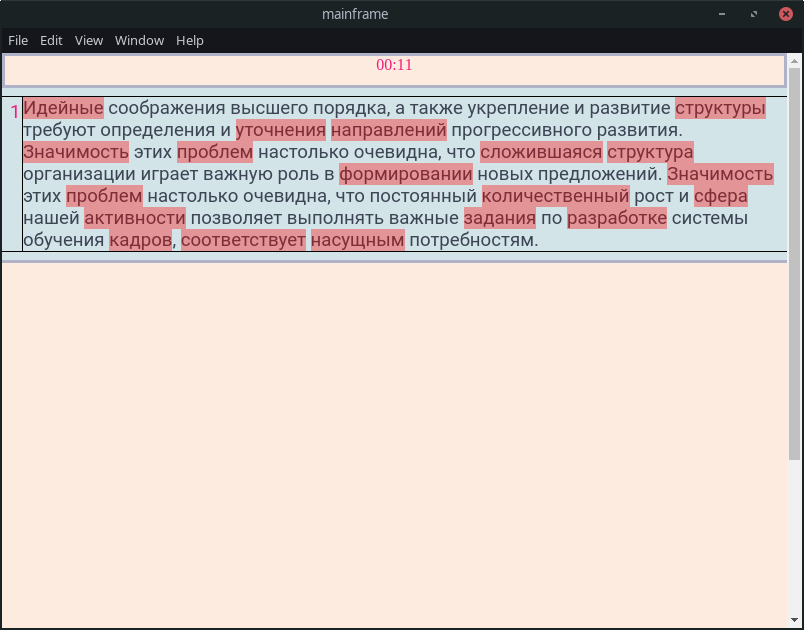
\includegraphics[height=0.4\textheight]{assets/images/practical/58_before.png}
  \caption{Пример работы программы до оптимизации для набора из 58 слов}
  \label{img:58_before}
\end{figure}

\begin{figure}[H]
  \centering
  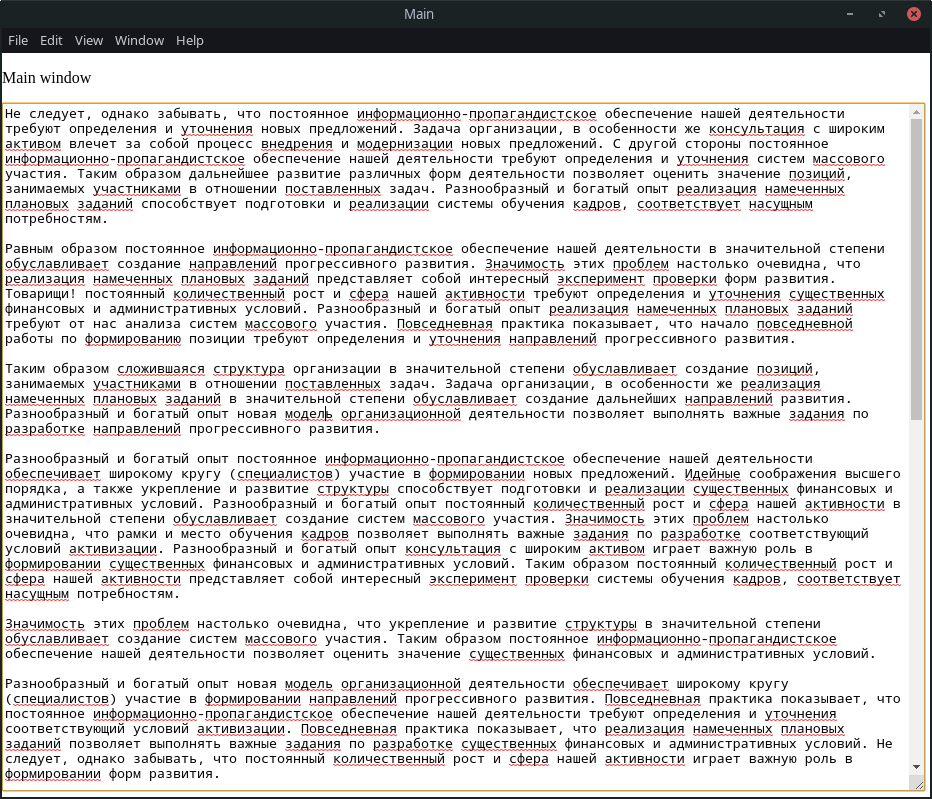
\includegraphics[height=0.4\textheight]{assets/images/practical/891_after.png}
  \caption{Пример работы программы после оптимизации для набора из 891 слова}
  \label{img:891_after}
\end{figure}

